% Asset ID: A21TrigonometricFunctionsTikZ-004
% Source: Chapter 6 inverse trig functions + CCEA A21-TRIG-LO002 and A21-TRIG-LO003
% Related lesson section: Inverse Trig Functions
% Purpose: Show that an inverse graph swaps domain and range after restricting the original graph.

\documentclass[tikz,border=8pt]{standalone}
\usepackage{amsmath}
\usetikzlibrary{positioning, arrows.meta, calc}
\begin{document}
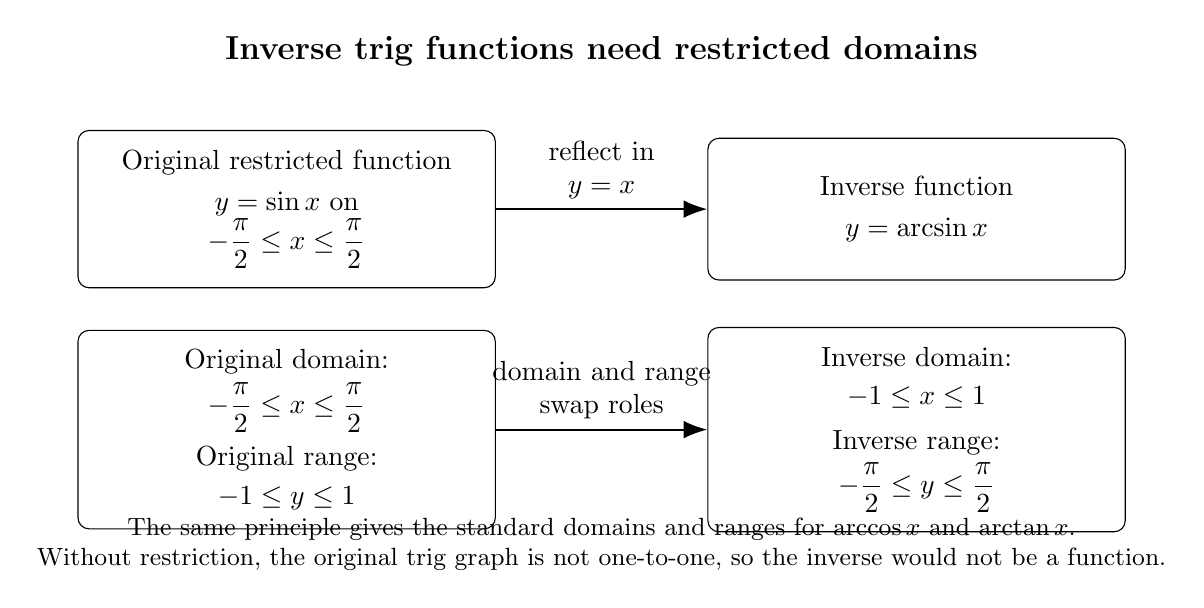
\begin{tikzpicture}[box/.style={draw,rounded corners,align=center,minimum width=5.3cm,minimum height=1.8cm,inner sep=7pt},arrow/.style={-{Latex[length=3mm]},thick},heading/.style={font=\large\bfseries},note/.style={align=center,font=\small}]
\node[heading] at (0,3.1) {Inverse trig functions need restricted domains};
\node[box] (original) at (-4,1.1){Original restricted function\\[3pt]$y=\sin x$ on\\$-\dfrac{\pi}{2}\le x\le\dfrac{\pi}{2}$};
\node[box] (inverse) at (4,1.1){Inverse function\\[3pt]$y=\arcsin x$};
\draw[arrow] (original) -- node[above,align=center]{reflect in\\$y=x$} (inverse);
\node[box] (domainrange) at (-4,-1.7){Original domain:\\[2pt]$-\dfrac{\pi}{2}\le x\le\dfrac{\pi}{2}$\\[4pt]Original range:\\[2pt]$-1\le y\le 1$};
\node[box] (swapped) at (4,-1.7){Inverse domain:\\[2pt]$-1\le x\le 1$\\[4pt]Inverse range:\\[2pt]$-\dfrac{\pi}{2}\le y\le\dfrac{\pi}{2}$};
\draw[arrow] (domainrange) -- node[above,align=center]{domain and range\\swap roles} (swapped);
\node[note, below=1cm of $(domainrange)!0.5!(swapped)$] {The same principle gives the standard domains and ranges for $\arccos x$ and $\arctan x$.\\Without restriction, the original trig graph is not one-to-one, so the inverse would not be a function.};
\end{tikzpicture}
\end{document}
